\section{IBM Roadmap on Quantum Computing\label{sec:ibm_roadmap}}

Bringing about useful quantum computing to the scientific world, and in particular, to the \gls{hep} community, is contingent on the development of quantum computing hardware and software that permits the execution of quantum algorithms at a scale that is capable of producing insights and results not accessible by classical computers. But more than only requiring a large-scale device, one requires that the components are sufficiently reliable and have coherence times as well as gate parameters of high quality~\cite{wack2021quality}. The IBM Quantum roadmap proposes a list of stepping stones that progressively improve on the necessary requirements. The first development roadmap was previewed in 2020~\cite{IBM_roadmap1} laying out a progression of the then available 27 qubits Falcon devices to the Condor chip with 1,121 qubits by the end of 2023. With the release of the 433 qubit Osprey chip a the end of 2022~\cite{OspreyIBMnews} the roadmap has been extended~\cite{IBM_roadmap2}. %c.f. FIG~\ref{fig:roadmap}. 
The new roadmap now lays out a path to the newly introduced Kookaburra chip with 4,105 qubits that utilizes interconnected chip designs with long-range couplers. Furthermore, the new roadmap added new chip architectures, such as the Heron chip with 133 qubits incorporating recent advances from gate and qubit research.
%
\begin{figure*}
    \centering
    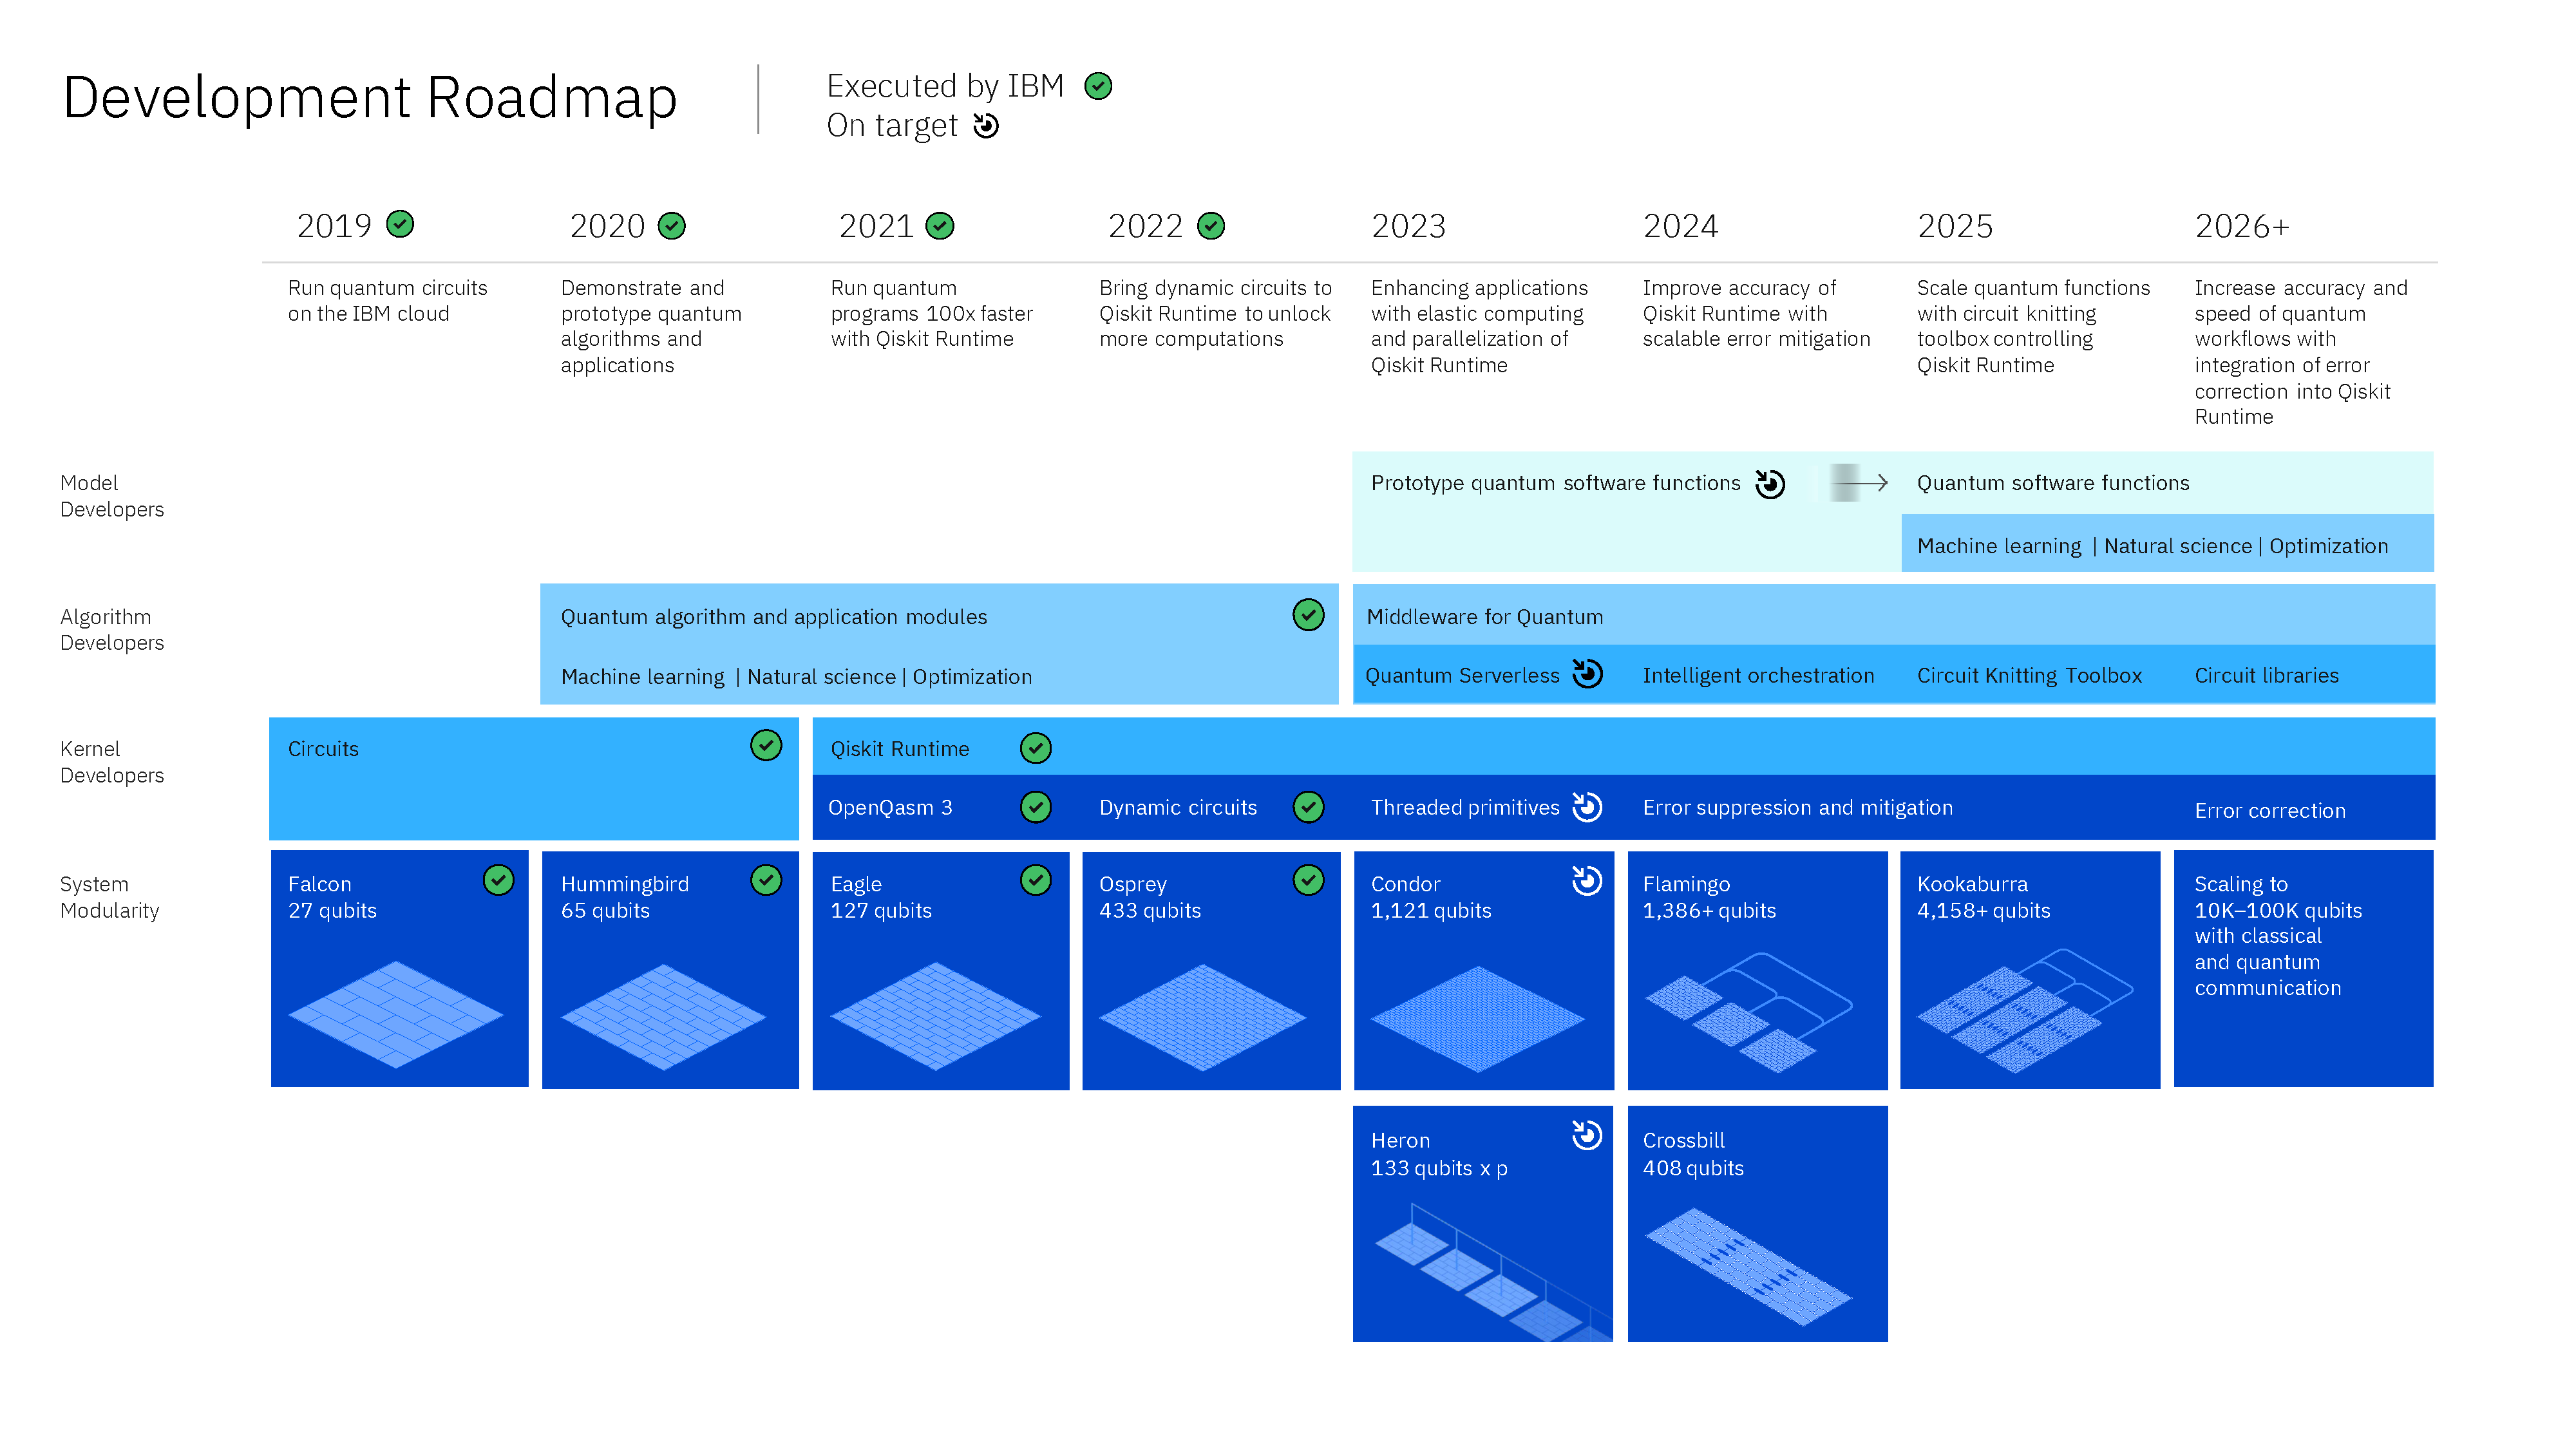
\includegraphics[width=0.95\linewidth]{roadmap_middleware.pdf}
    \caption{IBM's roadmap for upccoming quantum computers, updated 2022.}
    \label{fig:roadmap}
\end{figure*}

The greatest adversary to the realization of large-scale quantum computers is noise. The components of quantum computers are considerably more sensitive to imperfections and external interactions than their classical counterparts, leading them to decohere and turn into classical mixtures~\cite{unruh1995maintaining}. It is therefore almost universally accepted that complex and high-depth quantum algorithms such as Shor's factoring algorithm~\cite{shor1994algorithms}, quantum amplitude amplification~\cite{brassard1997exact,grover1998quantum}, phase estimation~\cite{kitaev1995quantum} or the long-time simulation of quantum dynamics will require quantum error correction. The design plans for the progressively larger \gls{qc} layouts are therefore aimed at providing a path to the long-term goal of realizing a fault-tolerant quantum computer. However, current error-correcting codes, which could be used to realize fault-tolerant quantum computing at a non-trivial scale, require system sizes that exceed the available hardware by several orders of magnitude~\cite{gidney2021factor,lee2021even}. Building a fault-tolerant computer, therefore, requires not only higher quality and larger scale devices but also research in error correcting codes. Recent advances in the theory of error correction~\cite{breuckmann2021quantum} provide us with reason to be optimistic about future progress. However, if we only wait for the realization of a fault-tolerant quantum computer to run algorithms and do not actively explore the potential of near-term devices, we will forgo a promising opportunity to obtain a computational advantage in the near future.

We are observing remarkable progress in quantum hardware. As the roadmap and the already completed milestones indicate, we are both building larger devices and can manufacture components with an order of magnitude improvement in two-qubit gate fidelities~\cite{Stehlik2021}. A quantum processing unit at the scale of the 65-qubit Hummingbird chip could implement circuits with a few thousand gates to a reasonable degree of accuracy without resorting to error correction when two-qubit gate fidelities of $99.99\%$ become available. Circuits of such a size can arguably no longer be simulated by exact methods on a classical computer. This suggests an alternative path of utilizing current and impending quantum devices~\cite{path_error_mit}. Here, one restricts to computations with only shallow-depth quantum circuits, where the size of the circuit is determined by hardware parameters such as coherence times and gate fidelities. As these parameters improve, the circuit sizes that become accessible increase, ultimately leading to circuits that provide a computational advantage over classical approaches. This path lays out a gradual progression to obtaining quantum advantage one hardware improvement at a time, ultimately driving the hardware evolution to progressively better and larger devices until error correction methods can be applied to provide us with access to circuits no longer limited by the device noise.

Early experiments~\cite{kandala2017hardware} demonstrated that despite the restriction to shallow-depth circuits, noise and decoherence lead to a bias in the estimates of expectation values. For this approach to provide an advantage over classical approximation methods this bias has to be mitigated. These observations have motivated the development of error mitigation tools such as \gls{zne}~\cite{Li2017Efficient,Temme2017Error} and \gls{pec}~\cite{Temme2017Error}. The goal of these methods is to reduce, or even fully remove, the noise-induced bias from expectation values measured in shallow-depth circuits. This is achieved by slightly modifying the circuits in different ways and combining measurement outcomes in post-processing to produce noise-free estimates. The protocols introduce an additional computational and sampling overhead that will ultimately grow exponentially in the noise strength, illustrating that these protocols do not extend the circuit depth beyond the device specific parameters, but only ensure that accurate values are produced within the allotted circuit size. The \gls{zne} method was experimentally implemented for the first time on small-scale chips~\cite{Kandala2019Error}. There it was shown that the effect of noise in earlier experiments~\cite{kandala2017hardware} could be removed. Recently it was demonstrated~\cite{Kim2022Scalable} that this method could be scaled to larger circuit sizes on improved quantum hardware, such as the recent version of the 27 qubit Falcon processor, by combining the method with error suppression techniques including dynamical decoupling~\cite{viola1998dynamical,viola1999dynamical} and Pauli - twirling~\cite{Bennett1996Purification,KnillFault2004,Kern2005Quantum}. Advances in learning and modelling correlated noise on quantum processors have enabled the implementation of \gls{pec}~\cite{Berg2022Probabilistic} to fully remove the noise bias for even the highest weight observables on larger devices.

To enable the scientific community to utilize these advances, IBM Quantum has announced a challenge to both internal developers as well as the community: the $100\otimes 100$ Challenge~\cite{IBM_100by100}. In 2024, IBM Quantum is planning to offer a quantum computing chip capable of calculating unbiased observables of circuits with 100 qubits and 100 depth of gate operations in a reasonable runtime, i.e. within a day. This new tool is to challenge the community towards proposing quantum algorithms that utilize this hardware to solve interesting problems, which are notoriously hard for classical computers. 

The \gls{hep} community plays a pivotal role here since the field is one of the driving sources for challenging computational problems inherent to quantum mechanics. This community is ideally equipped to propose problem relevant heuristics~\cite{RevModPhys.94.015004,Preskill2018} that stand to benefit from early demonstrations on quantum hardware 

%\noindent \textcolor{red}{Kristan, Ivano - end }    
%\noindent \textcolor{red}{Kristan - end}